
%----------------------------------------------------------------------------------------
%	CHAP introduction
%----------------------------------------------------------------------------------------

\chapterimage{blue-chapter-head_4-reduced.pdf} % Chapter heading image

\chapter{Tables}\label{chap:Tables}
\section{Overview}
Before you start an analysis, you will need to define Table nodes that will represent the data files needed in the analysis. MetaR explicitly represents files that contain tables of data. This is done so that you can easily refer to these tables, without having to remember where the file is located on your computer. 

\noindent In this Chapter, you will learn how to 
\begin{enumerate}
	\item define a MetaR table,
	\item  adjust the types of the columns of the data described in the file,
	\item annotate a table with groups,
	\item link groups in column group usage.
\end{enumerate}

\section{Create a Table}
To create a Table, right-click on a model in the project tab and select \menu{right-click > New > o.c.metar.tables > Table}. This will create an empty table, as shown in Figure~\ref{fig:NewTable} 

Tables have a name, a pathToResolve attribute and a list of columns. The following paragraph describe these attributes.
\paragraph{name}
The table name is set automatically from the path when you use the file selection button. You can change the name to match your analysis needs and make it easier to remember what is in the table.
\paragraph{path to resolve}
This attribute contains a path to the TSV file that you wish to analyze. The path may contain references to path variables that will be automatically resolved before MetaR attempts to load table information from the path. Path variable references can be written as \texttt{\${a.b.c}/data/file.tsv}. Such a reference will require you to define the a.b.c path variable name and associate it with a value on each machine where the table will be used. You can define path variables with the Preferences/Settings MPS menu (\menu{MPS > Preferences> PathVariables} on Mac, \menu{MPS > Settings > PathVariables} on PC).

\paragraph{columns}
Columns is an attribute that presents the list of columns identified in the TSV file. Each column has a name, a type, and may be annotated with a set of column groups (see Section~\ref{sec:ColumnGroups} for details about column groups).
MetaR supports the following column types, which map to the R data types:
\begin{enumerate}
	\item \textbf{Numeric}. Any number. Technically, can be a floating number or an integer.
	\item \textbf{String}. A string of character.
	\item \textbf{Boolean}. A type that can only have two values: \texttt{true} or \texttt{false}.
	\item \textbf{Category}. A type that can take only a limited number of values (e.g., \{\texttt{RED}, \texttt{GREEN}, \texttt{BLUE}\} would be a category with three values, \texttt{RED}, \texttt{GREEN} and \texttt{BLUE}.
\end{enumerate}
These types are automatically determined from the data in the table file. However, in case the automatic algorithm failed for a table, you can change the types manually. To do this, put the cursor over the name of the type in the column section, and use auto-completion in the inspector to change to the desired type.
 
\begin{SCfigure}
  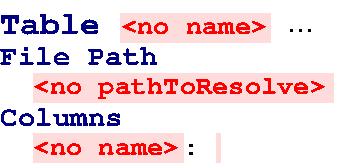
\includegraphics[width=\figWidthTiny]{figures/NewTable.pdf}
  \caption[New Table.]{\textbf{New Table.} This figure presents a freshly created Table AST Root node. You can use the button located to the right, after the <no name> red label, to open a file selection dialog. Use this dialog to locate a TSV file to configure this table.}
\end{SCfigure}\label{fig:NewTable}

\section{Column Groups}\ref{ColumnGroups}